% 第 4 章 系统测试与结果
% 本章引用键（实际使用）：fips203, kyberslash, clangover, dudect, rtlf, microwalk, binsec
% 图表按章编号：本章表 4.1–4.7，图 4.1–4.6
% 图 4.2 为关键函数反汇编对比，90 格数据保留为表 4.4

\section{系统测试与结果}

本章按“核心结论 → 支撑数据 → 原因分析”组织。四个核心结论：（1）M1 与 M4 在防护前后实现“可区分 → 不可区分”的完整对照（4.3、4.6 节）；（2）M2 定位层命中、计时层未检出，两者分属不同证据层（4.4、4.5、4.12 节）；（3）M5 阴性对照在既定预算下未检出且未误报（4.3、4.5、4.12 节）；（4）结论只对指定产物与预算成立，跨环境与网络结论不混用（4.10、4.11 节）。各节先给结论，再列数据，最后解释原因。

\subsection{测试方案与环境}
% A-30 计时精度与环境
% A-31 运行批次
% A-26 优化级别
% A-01 M1 主结果
% B-08 运行批次合计

测试分六组，每组回答题面条目中的一个问题。环境是一台 x86\_64 裸金属，所有时间结论只在这台机器上成立。六组是功能与语义等价、检测与定位、防护复测、功效与稳健性、性能、跨环境与多工具。分组按”回答哪一个问题”划分，不按工具划分；同一份原始数据可在不同组里被引用。

六组与题面的对应关系：功能与语义等价对应第 1 条，检测与定位对应第 3--5 条，防护复测对应第 6、7 条，功效与稳健性对应第 4、8 条，性能对应第 8 条，跨环境与多工具对应第 9、11 条。第 2、10 条贯穿所有组。

实验采用绑核、关闭睿频、请求固定 4.30 GHz、性能调速策略、窗口外预热 100 次、输入随机交错，并将分配与 I/O 移出计时窗口。表~\ref{tab:env} 给出七项环境要素。处理器、操作系统、编译器、动态分析、形式化、计时源与频率控制各自固定。处理器行标注 SMT（同步多线程）开启、未配置 isolcpus（Linux 内核的 CPU 隔离参数）。换掉其中任何一项，时间结论都要重测。% A-30

\begin{table}[H]
\centering
\caption{测试环境}
\label{tab:env}
{\small
\begin{tabularx}{\textwidth}{|>{\raggedright\arraybackslash}p{2.3cm}|>{\raggedright\arraybackslash}X|}
\hline
项目 & 配置 \\
\hline
处理器 & AMD Ryzen 9 9950X（x86\_64），SMT 开启，未配置 isolcpus \\
\hline
操作系统 & Ubuntu 24.04.4 LTS，Linux 6.17，amd\_pstate 频率驱动 \\
\hline
编译器 & clang 18.1.3（主构建）。gcc 13.3.0 已安装但未用于对照实验 \\
\hline
动态分析 & Valgrind 3.22.0（Memcheck）。Valgrind 3.25.1 + KyberSlash varlat 补丁。Intel Pin 3.28（Microwalk 的插桩引擎） \\
\hline
形式化 & Binsec 0.11.3（关系符号执行）与 Z3 4.15.3（SMT 求解器） \\
\hline
计时源 & 单调时钟（完整解封装）。原始单调时钟（M4 比较调用） \\
\hline
频率控制 & 关闭睿频，性能策略，频率上下限均为 4,300,000 kHz，绑核 CPU2 / CPU6 \\
\hline
\end{tabularx}
}
\end{table}

表~\ref{tab:env} 汇总本次实验使用的处理器、编译器、工具版本与频率工作点。

操作系统与频率驱动最容易被忽略：锁频协议通过 sysfs 写频率上下限，换内核或换驱动，20 次探针的读数就可能落在不同工作点。编译器版本同样是背景信息：M1 的分支是 clang 18 在特定选项下的产物，换编译器等于换被测对象。环境表的作用是让“未检出”有明确的工具边界。

表~\ref{tab:matrix} 把五个模块、三类对象与七类实验环境排在同一张矩阵上。矩阵的行是实验类别，列是模块。空格按该模块在该类实验中没有对象或不适用登记。

\begin{table}[htbp]
\centering
\caption{实验矩阵与运行批次}
\label{tab:matrix}
{\footnotesize
\renewcommand{\arraystretch}{1.18}
\begin{tabularx}{\textwidth}{|>{\raggedright\arraybackslash}p{2.45cm}|*{5}{>{\centering\arraybackslash}X|}}
\hline
\textbf{维度} & \textbf{M1} & \textbf{M2} & \textbf{M3} & \textbf{M4} & \textbf{M5} \\
\hline
对象类别 & 真实历史 & 真实历史 & 人工校准 & 人工校准 & 阴性对照 \\
\hline
主类对家族 & 3 次 $\times 10^4$/类 & 3 次 $\times 10^4$/类 & 3 次 $\times 10^4$/类 & 3 次 $\times 10^4$/类 & 3 次 $\times 10^4$/类 \\
\hline
定位层 & 反汇编、Memcheck & varlat、反汇编 & Memcheck、Microwalk & Memcheck、Binsec & Memcheck、varlat、Binsec \\
\hline
90 格排查 & 30 格 & 30 格 & — & — & 30 格 \\
\hline
优化级别 & 4 级 $\times$ 2 版 & — & — & — & 4 级 \\
\hline
aarch64 & 4 级 $\times$ 2 版 & — & — & — & 4 级 \\
\hline
WSL2 虚拟化 & 4 级 $\times$ 2 版 & — & — & — & 4 级 \\
\hline
同机网络 & 2 版 $\times$ 2 次 & — & — & — & 2 次 \\
\hline
性能开销 & 解封装 & 解封装 & 解封装 & 小内核 & 解封装 \\
\hline
工具矩阵 & 6/9 种 & 6/9 种 & 6/9 种 & 6/9 种 & 7/9 种 \\
\hline
\end{tabularx}
}
\par\smallskip
{\footnotesize 运行批次：平台家族 54 次 + M2 微基准 6 次 + 收尾 117 次 = 177 次控制器运行。表中每一项实验均在运行台账中绑定了二进制摘要、随机数种子、绑定核心与对应的证据层级。}
\end{table}

矩阵每格绑定产物摘要、种子、CPU 与判定层；矩阵之外的组合没有数据。

正式采集分三批：平台家族 54 次控制器运行、M2 微基准 6 次、收尾 117 次（格式破损 18、性能 54、优化级别 36、锁频对照 9），合计 177 次。每次运行都经过计划校验、频率放行与退出恢复。M1 封存数据不计入 177 次，统计口径仍按当时冻结的家族。% A-31 % B-08

被拒绝的运行与未执行项分开登记。优化级别实验中有 1 次运行因 20 次探针的频率跨度 54,629 kHz 超过 50,000 kHz 阈值被控制器拒绝，换名重跑后计入。性能批次有 1 次运行跨度 50,310 kHz 略超阈值，20 个采样值仍在 ±2\% 带内，已如实登记。逐次实测中位频率的中位数为 4,309,722.5 kHz，相对名义 4.30 GHz 的偏差为 +0.005\%（按逐次运行中位频率的中位数与名义值比较，不是单次采样）。异常样本判定规则：控制器拒绝（频率探针超带或跨度超阈）、参数错误、客户端缺失等无计时值的记录单列为失败尝试；有计时值的调用全部保留（含普通长尾），不按分位数截尾；稳健性结论另行独立给出。未执行项包括 GCC 对照、-O1/-Oz/-Og 三个优化级别、额外架构、isolcpus 与关闭 SMT、Microwalk 扩展到 M1/M2、Binsec 覆盖完整解封装、面向 CI 的回归门禁。它们在第 6.2 节按影响范围说明，与阴性分开统计。% A-26 % A-31
M1 数据来自前期封存批次，引用时单独标注，不与 M2--M5 合并。% A-01

\subsection{功能与语义等价测试}
% A-33 M1 功能向量
% A-34 M2/M3/M5 功能向量
% A-35 修复等价与额外输入

在开展侧信道分析与代码防护前，首先必须验证各被测实现的密码学功能正确性，并确保修复前后的输入输出逐字节一致（不改变算法安全语义）。由于三个真实实现对应的标准演进阶段不同——M1 对应 FIPS 203 初始公开草案（IPD），M2 对应 NIST 第三轮 Kyber768 参考实现，M5 对应 FIPS 203 正式标准——测试时需分别采用各自版本对应的官方测试向量（KAT）。\cite{fips203}
表~\ref{tab:function} 把五组功能结果列在一起。% A-33--A-35

\begin{table}[H]
\centering
\caption{功能正确性与语义等价}
\label{tab:function}
{\small
\begin{tabularx}{\textwidth}{|>{\raggedright\arraybackslash}p{2.5cm}|>{\raggedright\arraybackslash}p{3.5cm}|>{\raggedright\arraybackslash}X|}
\hline
对象 & 测试向量 & 结果与说明 \\
\hline
M5、M3 & NIST 独立向量 & 各 80/80（含隐式拒绝用例） \\
\hline
M1 两版 & NIST ACVP（自动密码算法验证程序）转换的 ML-KEM-768 向量 & Encaps 25/25（100\%）、Decaps 10/10（100\%，含隐式拒绝）全部通过；KeyGen 25 例用于验证 FIPS 203 初始公开草案（IPD）与正式版在 K-PKE.KeyGen 哈希域分隔字节上的标准演进差异。另有 20 例密钥校验因封装层无对应入口记为不适用 \\
\hline
M2 两版 & Kyber round3 官方 KAT & 100/100。普通构建与 ASan/UBSan（地址与未定义行为消毒器）构建测试各 7/7 \\
\hline
修复等价性 & 同一驱动、同一公开输入 & 三对“未修 / 已修”实现的逐例输出摘要 diff 全空 \\
\hline
额外输入 & 一半随机密文、一半逐字节篡改 & 隐式拒绝 1000/1000 按 FIPS 203 或 round3 规范生效 \\
\hline
\end{tabularx}
}
\end{table}

KeyGen 向量用于核验 FIPS 203 标准演进。liboqs 0.10.0 实现的是初始公开草案，草案的 K-PKE.KeyGen 哈希输入没有最终版新增的参数集域分隔字节，因此与最终版向量不同属于标准口径差异，记录为。

60 例包括 Encaps 25 例、Decaps 10 例和用于标准演进差异核验的 KeyGen 25 例；其中 Encaps 与 Decaps 均全部通过。另有 20 例密钥校验因封装层没有对应入口，单列为不适用，不计入这 60 例。
这 20 例不适用是因为封装层没有对应入口；该状态与向量执行结果独立记录，避免混淆接口覆盖与算法正确性。

M2 用 Kyber round3 官方 KAT，100/100。普通构建与 ASan/UBSan 构建各 7/7。M3 与 M5 用 NIST 独立向量，各 80/80，含隐式拒绝用例。三套对象的向量来源不同，是因为它们的标准版本不同：M2 是历史 Kyber768，只能用 round3 的 KAT。M5 对应最终标准，用 NIST 向量。M3 基于 M5 基线，向量与 M5 同源。把三套向量混在一起统计“总通过率”没有意义，表~\ref{tab:function} 因此按对象分行。

三对未修/已修实现的逐例输出摘要 diff 全空，说明修复没有改动算法语义。修复涉及三类改动：把分支改成掩码选择、把除法改成乘法与移位、把人工夹具的查表或提前返回改成固定路径。改动只落在执行路径上，不落在输出上。逐例摘要 diff 比“再跑一遍 KAT”更强：KAT 只比较最终共享密钥，摘要 diff 还把中间输出与返回码一起比较。任何一处字节变化都会留下痕迹。

1000 例额外输入（一半随机密文、一半逐字节篡改）中，隐式拒绝 1000/1000 记录。随机密文检验一般路径上的解析与拒绝，逐字节篡改检验比较逻辑在单个字节不同时的行为。两类输入都按公开输入处理，失败路径按规范返回假密钥。1000/1000 说明失败路径在修复后保持生效；失败路径与成功路径的耗时可区分性由 3.3 的计时层回答。

ASan/UBSan 构建的 7/7 是另一条证据。普通构建只证明功能正确，消毒器构建还要证明没有越界、未定义行为与内存错误。7/7 说明修复没有引入这类问题。消毒器构建的性能不适合计时，功能测试只在普通构建上做计时，两者分开登记。



\subsection{端到端可区分性}
% A-01--A-08 五模块主结果
% A-09--A-14 统计判定与 dudect
% A-16 RTLF
% B-01 效应占比
% B-04 RTLF 数据集
% B-07 主类对样本

预注册 Holm 家族中，只有 M1 未修复版主类对与 M4 脆弱实现（vulnerable版）被拒绝。M2、M3、M5 的家族均未拒绝任何检验。图~\ref{fig:forest} 把七个类对的均值差与 95\% 区间放在同一把尺子上：M1 未修复版与 M4 脆弱实现的区间不含 0，其余五个区间含 0。% A-01--A-08

\begin{figure}[htbp]
\centering
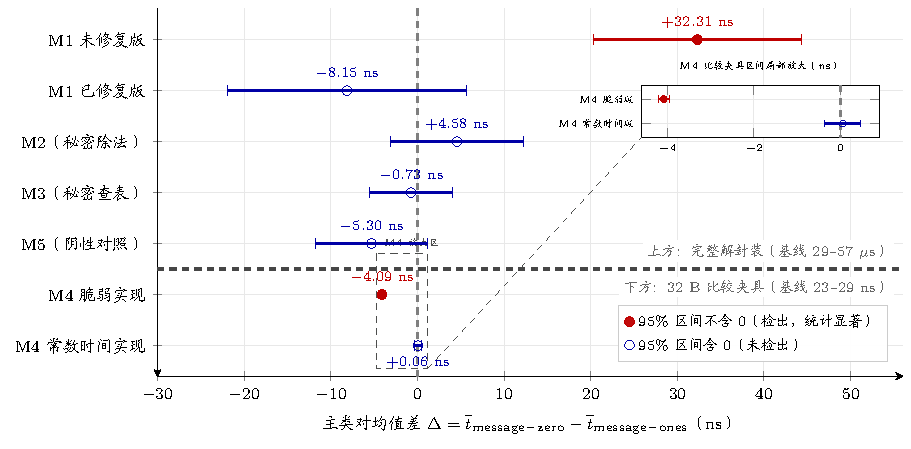
\includegraphics[width=0.98\textwidth]{assets/fig5.pdf}
\caption{五模块主类对均值差与 95\% 区间}
\label{fig:forest}
\end{figure}

家族的构成决定了门槛。M1、M2、M3、M4 各 6 项，M5 3 项。每个模块的 6 项来自 3 次独立运行 $\times$ 2 个版本或实现。Holm 是逐步下降校正：家族内 $p$ 值升序排列，第 $i$ 个与 $\alpha/(m-i+1)$ 比较，一旦某一步不拒绝就停止。M1 的 $m=6$，最小 $p$ 的门槛是 $0.05/6\approx0.00833$。M4 的 $m=6$，门槛相同。M5 的 $m=3$，门槛是 $0.0167$。门槛在采集前写进计划，不随观测到的 $p$ 值变化。

先看 M1。三次独立运行的均值差为 +39.337、+31.117、+22.337 ns，三个 95\% 区间都不含 0。逆方差合并为 +32.311 ns，区间 [20.282, 44.339]。Holm 家族 $m=6$，最小 $p=1.30\times10^{-5}$，低于阈值 0.00833，是家族中唯一被拒绝的检验。效应占完整解封装均值 57,010.7 ns 的 0.0567\%，约 0.06\%。32 ns 在 10 ns 的最小步进下只有 2--3 个分辨率单位，单次调用不可分辨，结论靠每类 10,000 次、三次运行。dudect 的最大 $t$ 为 26.41、40.64、14.92，RTLF 在未修版报告差异、在已修版未报告差异，方向与 Welch 检验一致。% A-01 % A-09 % A-11 % B-01 % B-07

三次运行的方向一致，比单次拒绝更重要。三次分别换种子、换物理核：同核不同种子两次，同种子不同核一次。三次都给出正号、区间都不含 0，说明结论与输入及物理核的局部状态无关。三次方向若不一致，即使合并后拒绝零假设，也按预注册规则登记为不稳定，结果以全部三次为准。M1 的三次结果没有触发这条规则。

效应大小与统计判定分属两个读法：32.311 ns 只占 57,010.7 ns 的 0.06\%，在绝对值上很小。它的统计判定来自每类 10,000 次、三次运行与预注册家族；拒绝零假设表示均值差与零可区分，效应大小按绝对值单独描述。这个效应在单次调用上不可分辨，在本地锁频、大样本下才可分辨。

M4 的阳性更强。脆弱实现（vulnerable版）三次运行的原始 $p$ 为 0、$9.23\times10^{-25}$、$3.14\times10^{-22}$，其中 0 为双精度下溢。Holm 家族 $m=6$，拒绝 3 项，均来自脆弱实现。合并差 $-4.089$ ns，区间 [$-4.215$, $-3.963$]；常数时间实现（ct版）合并差 +0.055 ns，区间 [$-0.363$, 0.473]，三次原始 $p$ 均不拒绝。dudect 最大 $t$ 从 356.6、396.9、395.6 降至 2.06、1.90、2.27。% A-06 % A-07 % A-10 % A-12

值得注意的是，图~\ref{fig:forest} 中 M4 的置信区间极窄，这是因为它仅测量单次 32 字节比较函数（基准耗时约 23～29 ns），不包含多项式数论变换（NTT）、采样与序列化等耗时操作，背景噪声远小于完整解封装（基准耗时 29～57 $\mu$s）。在相同的每类 10,000 次样本下，M4 的最小可检测效应（MDE）低至 0.19～1.19 ns，因此尽管其绝对时间差（$-4.089$ ns）仅为 M1（$+32.311$ ns）的八分之一，信噪比和统计显著性反而更高。这也说明，时间侧信道的可检出性同时取决于泄漏时延的绝对大小与被测窗口的背景方差。

M2 的家族没有拒绝项。完整解封装合并差 +4.58 ns，区间 [$-3.08$, 12.25]，含 0。按版本描述，未修版 +12.35 ns、已修版 $-11.20$ ns，$I^2=58.3\%$。两个版本方向相反且运行间一致性较弱，尚不能将差异归因于除法。按版本合并值不属于预注册的 6 个家族成员。家族成员是三次运行的逐次检验，按版本值只作描述。

主类对按解密消息位设计：message-zero 与 message-ones 只让解密消息的位不同，除法的被除数是否随消息位系统变化按输入设计登记。这一条在 4.7 的检测预算里再展开。M2 的 dudect 阳性落在已修版（4.68、3.05、3.66 对 36.27、30.94、61.91），记录为。4.12 把它作为单工具误读的例子。% A-03 % A-04 % A-13

M2 的未修版描述性合并区间为 [2.98, 21.71] ns，虽不含 0，却不属于采集前规定的六个逐次检验。判定以采集前规定的六个逐次检验为准，事后合并按描述性参考登记。$I^2=58.3\%$ 表示运行间差异较大，漂移的具体来源按输入与环境登记。

M3 的合并差为 $-0.73$ ns，区间 [$-5.56$, 4.10]，Holm 家族未拒绝 0。M5 的合并差为 $-5.30$ ns，区间 [$-11.77$, 1.16]，家族 $m=3$，拒绝数为 0。M3 是人工夹具，开启查表版（on版）与消除查表版（off版）只差人工查表，计时层未能分辨该机制。M5 的 dudect 最大 $t$ 为 2.10、1.98、2.82，低于阈值 10。% A-05 % A-08 % A-14
M5 的三个家族成员均未接近拒绝门槛，作为阴性对照与其余模块形成对比。

$\Delta=\bar t_{C_0}-\bar t_{C_1}$：正值表示全 0 消息类较慢，负值表示全 1 消息类较慢。


图~\ref{fig:forest} 按模块排列主类对均值差与置信区间，M4 的两种实现相邻列示，便于比较其定位与计时结果。

族外检验给出另一层信息。RTLF 在 $\alpha=0.01$、固定种子与 10,000 次 bootstrap 的设置下，对 M2--M5 的 42 个数据集给出 30 个未检出、12 个检出。检出的 12 个集中在 M2 主类对与 M4 脆弱实现（vulnerable版）及其对照，M3 的 12 个与 M5 的 6 个数据集全部未检出。RTLF 与 Welch 检验比较的对象不同：前者比较分布与分位，后者比较均值。两者不互相替代，也不并入同一个 Holm 家族。\cite{rtlf} % A-16 % B-04

族外检验按独立口径登记，原因是零假设与错误控制方式不同：RTLF 用 bootstrap 控制第一类错误，dudect 用最大 $t$ 的经验阈值，Mona 用箱体分离。并入同一个 Holm 家族会得到介于 0.05 与 0.01 之间的混合错误率。它们的位置是交叉印证：同向时增加信心，反向时提示输入类或环境有问题，每次结果按检验类型解读。

dudect 也属于族外。它用在线 $t$ 检验，阈值是上游默认的 10，不转换成 $p$ 值参与 Holm。M1 未修复版在三批内停止并报告泄漏，已修跑满批次仍为“可能常数时间”。M4 脆弱实现三次都报告泄漏，常数时间实现（ct版）三次都未报告。M5 三次都未报告。\cite{dudect}

主类对是同一份确定性密文的 10,000 次重复，单次运行的区间反映测量噪声；密文间的变异由跨种子复测覆盖。10 ns 的量化尺度下，32 ns 的效应只有 2--3 个分辨率单位，这解释了为什么必须用大样本与预注册家族。图~\ref{fig:forest} 仅呈现均值差与区间；机制归因结合 4.4 节的函数定位证据。



\subsection{函数级泄漏定位}
% A-17 M1 定位
% A-18 M2 定位
% A-19 M3 定位
% A-20 M4 定位
% A-21 M5 定位
% A-23 残留分支

定位层把每个阳性落到函数、指令或源码行。定位阳性与计时阳性是两件事，必须分开登记。同一个模块可以在定位层阳性、在计时层未检出，M2 就是这种组合。反过来，计时层阳性也必须能回到一条具体指令，否则无法判断修复是否生效。

动态检查的工作方式决定了它能回答什么。秘密标记把私钥中参与解密的 1152 B 与隐式拒绝秘密的 32 B 标成“未初始化”，公开输入保持已初始化。程序在标记下跑完整解封装，工具报告“以秘密值为分支条件”与“以秘密值为访存下标”两类事件。Valgrind 报告中的 errors 是运行期间该敏感指令被触发的累计次数，contexts 是该问题对应的独立代码位置（调用栈）数量。例如循环执行 256 次触发同一条敏感分支，会记为 256 errors / 1 context。报告里同时给两个数，分别呈现“执行次数”与“问题分布”。

M1 未修复版的消息编码函数中，\texttt{bt} 测试秘密消息位，\texttt{jae} 根据该位决定是否跳过系数写入，因此执行路径直接依赖秘密。私钥标记下，Memcheck 报告 1 个秘密条件跳转。官方修复版用 \texttt{setb} 将测试结果转为寄存器中的 0 或 1，再调用 16 位条件传送函数 \texttt{cmov\_int16}，通过取负、异或和按位与完成选择。反汇编里条件跳转消失，Memcheck 报告 0。两版的功能输出逐字节相同，说明消失的是执行路径，语义保持不变。\cite{clangover} % A-17

反汇编上的差别可以逐条读。未修版本是“按位测试 + 条件跳转”：测试结果决定是否跳过写系数。修复版本是“按位测试 + 置位 + 调用条件传送辅助函数”：测试结果被转为 0 或 1，辅助函数用取负、异或、与、再异或完成选择，不产生依赖秘密的跳转。修复前后的指令序列不同；修复后的选择不再通过秘密相关跳转完成。修复的代价是多了几条算术指令与一次调用，收益是分支消失。

\par\smallskip\noindent\textbf{M1 工具命中汇总：}反汇编与 Memcheck 双工具验证，未修复版定位到消息编码函数 1 处秘密条件跳转，修复后分支消失。

M2 的三处整数除法分别落在消息解码、多项式压缩与向量压缩。未修版本在可变时延检查下报告 1280 errors / 3 contexts。修复版本用乘法与移位替代除法，除法计数从 3 降到 0，可变时延报告 0/0。关闭可变时延检查时，两版都报告 0，说明普通 Memcheck 看不到除法：它只检查秘密是否进入分支或访存下标，不检查指令时延是否随操作数变化。1280 次错误来自同一源码位置的多次执行，3 个上下文才是问题分布。\cite{kyberslash} % A-18

三处除法各自对应一个上下文：消息解码一处、多项式压缩一处、向量压缩一处。三处的被除数都来自解密消息或重加密中间值，除数都是公开模数。修复用乘法与移位替代除法，三处的除法计数同时降到 0。varlat 的 1280 次错误分布在三个上下文上，说明三处都被执行到。如果只修一处，另外两处仍会报错。

\par\smallskip\noindent\textbf{M2 工具命中汇总：}varlat 工具定位到 3 处秘密相关整数除法，修复后计数归零；普通 Memcheck 无分支类命中。
图~\ref{fig:disasm} 汇总了 M1 的消息位选择和 M2 三处除法在实际编译产物中的指令形态。

\begin{figure}[H]
\centering
\noindent\begin{minipage}{0.96\textwidth}
\hrule
\vspace{0.4em}
\textbf{M1：\texttt{poly\_frommsg} 的消息位选择}
\par\smallskip
\begin{minipage}[t]{0.29\textwidth}
\textbf{x86\_64 未修版}
\begin{lstlisting}[numbers=none,frame=single,basicstyle=\ttfamily\tiny,columns=fullflexible,keepspaces=true,xleftmargin=0pt,escapeinside={@@}]
0x16e: @\textbf{bt}@  %ecx,%r8d
0x172: @\textbf{jae}@ 0x179
// 秘密比特决定是否跳转（关键差异指令）
\end{lstlisting}
\end{minipage}\hfill
\begin{minipage}[t]{0.29\textwidth}
\textbf{x86\_64 已修版}
\begin{lstlisting}[numbers=none,frame=single,basicstyle=\ttfamily\tiny,columns=fullflexible,keepspaces=true,xleftmargin=0pt,escapeinside={@@}]
0x39e9: bt   %r13d,%eax
0x39ed: @\textbf{setb}@ %dl
0x39f8: @\textbf{call}@ cmov_int16
// 无秘密分支的掩码选择（关键差异指令）
\end{lstlisting}
\end{minipage}\hfill
\begin{minipage}[t]{0.29\textwidth}
\textbf{aarch64 未修版}
\begin{lstlisting}[numbers=none,frame=single,basicstyle=\ttfamily\tiny,columns=fullflexible,keepspaces=true,xleftmargin=0pt,escapeinside={@@}]
0x4b6c: @\textbf{sbfx}@ w11,w11,#0,#1
0x4b70: @\textbf{and}@  w11,w11,w10
0x4be4: @\textbf{csel}@ w11,wzr,w10,ge
// 条件选择，不改变控制流（关键差异指令）
\end{lstlisting}
\end{minipage}
\par\smallskip
\textbf{M2：三处秘密相关除法在修复前后}
\par
{\scriptsize
\begin{tabularx}{\textwidth}{|>{\raggedright\arraybackslash}p{2.35cm}|>{\raggedright\arraybackslash}X|>{\raggedright\arraybackslash}X|}
\hline
函数 & 未修版（\texttt{\textbf{div}}） & 已修版（乘法与移位） \\
\hline
\texttt{poly\_tomsg} & \texttt{0x1877: \textbf{div} \%r9d} & \texttt{0x185f: \textbf{imul}；0x186d: \textbf{shr}} \\
\hline
\texttt{poly\_compress} & \texttt{0x16db: \textbf{div} \%r8d} & \texttt{0x16d5: \textbf{imul}；0x16e1: \textbf{shr}} \\
\hline
\texttt{polyvec\_compress} & \texttt{0x1a7f: \textbf{div} \%r8d} & \texttt{0x1a74: \textbf{imul}；0x1a7e: \textbf{shr}} \\
\hline
\end{tabularx}
}
\vspace{0.4em}
\hrule
\end{minipage}
\caption{关键函数编译产物反汇编对比。注：图中 M2 地址为模块局部偏移，附录表 D2 中地址为完整驱动链接后的虚拟地址，二者对应同一机器码；关键差异指令（\texttt{bt}/\texttt{jae}、\texttt{div}、\texttt{sbfx}/\texttt{and}/\texttt{csel} 等）加粗标注。}
\label{fig:disasm}
\par\smallskip
{\footnotesize M1 未修复版片段来自锁频归档对象，已修片段来自主构建 x86\_64 链接 ELF，aarch64 片段来自 aarch64 原生 ELF；M2 片段来自 KyberSlash Clang 18 -Oz 产物。地址均属于各自归档产物。}
\end{figure}

可变时延检查的边界也要写清楚。它标记“秘密操作数进入可变时延指令”；“这条指令一定产生可测差异”由计时层回答。除法在 x86\_64 上的时延是否随操作数变化，取决于处理器微架构、操作数大小与流水线状态。工具指出“这里有秘密操作数”，泄漏量级由计时层评估。M2 的定位阳性与计时未检出按两层登记：前者是机制层，后者是端到端层，两层的判据不同。

M3 的 Memcheck 报告 1280 errors / 2 contexts，全部落在人工插入的秘密下标读取。消除查表版（off版）去掉查表后为 0/0。Microwalk 在同一对象上给出互信息 1.922 bits，是全场最高。消除查表版（off版）为 0.722 bits。Microwalk 只有 5 个公开 testcase、没有重复、没有统计检验，互信息只作定位层的独立佐证，不升级为泄漏量。\cite{microwalk} % A-19

互信息 1.922 bits 的含义是“看过这条指令的访存地址后，对秘密的不确定性平均减少 1.922 bit”。它按关联强度登记；泄漏量由计时层评估。1.922 bits 与“恢复多少位密钥”之间按可利用性分层登记。Microwalk 的 5 个 testcase 只覆盖 5 组公开输入，没有重复、没有统计检验。互信息高说明这条指令与秘密关联强；可利用性由攻击可行性分析回答。

\par\smallskip\noindent\textbf{M3 工具命中汇总：}Memcheck 定位到 2 处人工插入的秘密下标读取（1280 次命中），Microwalk 给出 1.922 bit 互信息峰值；消除查表后报告归零。

M4 的 Memcheck 报告 32 errors / 1 context，落在提前返回的比较行。Binsec 在同一对内核上判脆弱实现为 insecure，反例地址对应提前返回行；常数时间实现（ct版）判 bounded secure，路径探索完整。搜索深度限为 5 时，工具返回 unknown，而进程退出码仍是 0。M4 只开启控制流与访存检查，未开乘除法检查。\cite{binsec} % A-20

Binsec 的反例地址对应提前返回行，说明工具找到了一条“从第几个字节开始不同”的秘密相关路径。常数时间实现（ct版）的 bounded secure 限定在入口、终点与公开长度 1--16 B 的范围内没有找到秘密相关路径；范围外的输入按边界外处理。深度限 5 的 unknown 是另一个边界：不安全与安全均未证明，退出码按工具输出登记。

\par\smallskip\noindent\textbf{M4 工具命中汇总：}Memcheck 定位到比较内核提前返回行（32 次命中），Binsec 验证判定脆弱版为 insecure 并给出反例，常数时间版判定 bounded secure。

M5 在三种动态模式下各做 10 次完整解封装：普通 Memcheck、关闭可变时延、开启可变时延，三者都是 0 errors / 0 contexts。重加密路径的 Binsec 检查中，比较步骤 1088/1088 条路径完成，消息编码 1/1 条路径完成，没有秘密相关控制流。同一配置下 M4 的脆弱内核报告 insecure，说明工具在这套配置里不会把已知脆弱代码判成安全。Binsec 只覆盖重加密比较与消息编码，不覆盖完整解封装的所有性质。% A-21

三种动态模式的分工不同：普通 Memcheck 看分支与访存下标，关闭 varlat 看同一组输入下是否有普通标记错误，开启 varlat 看除法等可变时延指令。三者都是 0/0，说明在这组输入上没有这三类问题；换一组输入时未执行路径按输入集登记。Binsec 的 1088/1088 与 1/1 是路径计数，覆盖范围为重加密比较与消息编码两个内核。

\par\smallskip\noindent\textbf{M5 工具命中汇总：}Memcheck、varlat 与 Binsec 交叉排查均无秘密相关分支或除法命中（0 错误）。

定位层的输出要归一化成同一种证据记录：工具与版本、输入集合、命中位置、上下文数、处置结论。同一位置被两类工具命中记两条证据，只有一类命中时保留但不升级为“确认”。归因要求同一位置至少在三次运行中的两次出现，且换种子后仍出现，只出现一次的命中记为“待复核”。

五类工具的回答范围可以排成一条链：反汇编回答“机器码里有没有目标指令形态”；运行时是否真的触发由秘密标记回答。秘密标记回答“秘密是否进入分支或访存下标”；可变时延指令由 varlat 回答。可变时延检查回答“秘密是否进入除法等指令”；缓存与分支由其他工具登记。轨迹互信息回答“哪些指令与秘密的关联最强”；时序可利用性由计时层回答。有界符号执行回答“给定范围内是否存在秘密相关路径”；范围外的行为按边界外处理。链条上的每一环各回答一个问题，合起来覆盖机制层的几个侧面。

定位层结论限于各工具的输入与检查范围；M4 只覆盖 32 B 比较夹具，Binsec 只覆盖给定内核和公开长度。定位阳性与计时阳性分开登记：M1 两层都阳性，M2、M3 定位阳性而计时未检出，M4 两层都阳性，M5 两层都未检出。

\subsection{泄漏源全流程排查}
% A-22 90 格汇总
% A-23 残留分支
% B-06 90 格分解

90 格排查把“六类来源 $\times$ 五个步骤 $\times$ 三个实现”逐格判定。5 个“存在”之外，还有一处更需要解释：官方修复后仍残留的同源分支。判定只有四种：存在、不存在、不适用、未检查。判“存在”必须给出可指认的函数、指令或源码位置以及触发它的输入。判“不存在”必须写明用了哪种检查、覆盖了哪些输入。判“不适用”要求该机制在这一步骤上不可能出现。判“未检查”单列，不并入阴性。

五个步骤是解密、哈希派生、重加密、比较与隐式拒绝。把哈希派生从重加密里拆出来，是因为哈希路径上的问题如果被记到重加密名下，定位只能停在“重加密有问题”这一层。拆开后，每一步都有自己的函数与指令，修复后可以逐格复查。六类来源是敏感分支、提前返回、可变时延指令、秘密下标、数据相关循环与异常路径。三个实现是 M1、M2 与 M5，人工夹具 M3、M4 不进入这张表，因为它们只覆盖单一机制，放进 90 格会把夹具结论与真实实现混在一起。


\begin{algorithm}[H]
\caption{90 格泄漏源排查}
\label{alg:sweep}
\begin{algorithmic}[1]
\Require 实现集合 $\{$M1, M2, M5$\}$。步骤集合 $\{$解密, 哈希派生, 重加密, 比较, 隐式拒绝$\}$。六类来源
\Ensure 90 格判定与证据
\For{每个实现、每个步骤、每类来源}
  \State 检查源码与反汇编
  \State 运行 Memcheck、varlat、Microwalk、Binsec（适用时）
  \State 判定：存在 / 不存在 / 不适用 / 未检查
  \State 记录函数、源码行或指令地址、证据编号
\EndFor
\State 汇总：存在 5 / 不存在 75 / 不适用 10 / 未检查 0
\end{algorithmic}
\end{algorithm}

算法~\ref{alg:sweep} 给出了 90 格矩阵在实际编译产物与多工具检测下的全流程逐项排查规程。表~\ref{tab:sweep} 给出汇总。分模块行按每模块 30 格减去存在与不适用导出，全表见附录 D（表 D1--D3）。% A-22 % B-06

\begin{table}[H]
\centering
\caption{全流程排查汇总}
\label{tab:sweep}
{\small
\begin{tabularx}{\textwidth}{|>{\raggedright\arraybackslash}p{3.7cm}|>{\raggedright\arraybackslash}p{1.0cm}|>{\raggedright\arraybackslash}X|>{\raggedright\arraybackslash}X|>{\raggedright\arraybackslash}X|>{\raggedright\arraybackslash}X|>{\raggedright\arraybackslash}X|}
\hline
实现 & 存在 & 存在格分布 & 不存在 & 不适用 & 未检查 & 小计 \\
\hline
M1 liboqs 0.10.0（未修 / 982c762） & 1 & 重加密 / 敏感分支 1 格 & 26 & 3 & 0 & 30 \\
\hline
M2 Kyber768（a621b8d / 272125f） & 3 & 解密 / 可变时延 1；重加密 / 可变时延 1；重加密 / 敏感分支 1 & 24 & 3 & 0 & 30 \\
\hline
M5 mlkem-native b3ba7b3 & $1^{*}$ & 隐式拒绝 / 提前返回 1 格$^{*}$ & 25 & 4 & 0 & 30 \\
\hline
合计 & 5 & 存在格集中在 M1、M2 的重加密与 M2 的解密步骤 & 75 & 10 & 0 & 90 \\
\hline
\end{tabularx}
\par\smallskip{\footnotesize \textbf{注：}$^{*}$M5 唯一“存在”格为解封装密钥中公开密钥数据的哈希完整性检查，属公开信息例外，记录为，不计作秘密相关泄漏。存在格逐格明细（函数、指令或源码位置与触发输入）见 4.5 节与附录 D。}
}
\end{table}

5 个“存在”逐格如下。M1 未修复版/重加密/敏感分支：消息编码函数中的按位测试后条件跳转，Memcheck 1 个上下文。M2 未修复版/解密/可变时延指令：消息解码中的整数除法。M2 未修复版/重加密/可变时延指令：多项式压缩与向量压缩中的整数除法。M2 未修复版与已修复版/重加密/敏感分支：消息编码函数中的同一分支在两版中都存在。M5/隐式拒绝/提前返回：上游设计行为，记录为。% A-22

表中这 5 处“存在”并非凭经验主观挑出，而是严格依据客观证据判定：只有同时定位到具体的函数、机器指令或源码行号，并能通过实际输入稳定触发时，才将该项记为“存在”。5 处命中项中，4 处位于历史漏洞实现 M1 和 M2；剩余 1 处位于 M5 的解封装密钥公开哈希完整性校验。由于该校验仅比较公开数据、不接触任何秘密信息，属于标准允许的公开检查逻辑，不构成侧信道漏洞。

表中记为“不适用”的 10 项，是指该类侧信道机制在对应算法步骤中从结构上不存在触发前提（例如纯算术运算与哈希派生步骤不涉及错误分支或异常退出机制），在附录 D 中均逐项注明了结构原因，与“已检查且未发现问题（不存在）”严格区分。% A-22

第 4 格呈现了全流程排查的超额发现：KyberSlash 官方修复提交消除了目标除法，但消息编码函数中的按位测试后条件跳转仍在。未修复版与已修复版的指令字节逐字节相同，秘密标记 Memcheck 在两版各报 256 errors / 1 context。该函数体与 M1 未修复版相同，即与 clangover 同源。主类对 message-zero 与 message-ones 使该分支在每个消息位上走系统性不同的路径，为 RTLF 在 M2 两版主类对上均报告分布差异、而格式破损对照未报告，提供了机制层候选解释。该发现把“修复目标除法”与“产物中所有秘密相关机制均已消失”区分开：机制是否全部消失须按 90 格逐格核验。这一发现补充了排查覆盖，尚未确定该分支对端到端耗时的独立贡献。\footnote{官方修复提交 272125f。另一提交 dda29cc 只修第一处。提交号仅用于定位历史版本。} % A-23

这一结果展示了全流程排查对单点补丁核验的补充作用：除法消失后，另一种秘密相关机制仍可能留在同一产物中。已修版三个种子的偏移分别为 +21.7、$-17.1$、$-15.5$ ns，Holm 拒绝数为 0；现有测量尚未分离代码布局和该分支的独立贡献，因此将其登记为解释 RTLF 分布差异的机器码层候选。% A-23
90 格记录均包含实现与产物摘要、步骤、来源类别、函数或指令位置、触发输入和检查手段，完整结果见附录 D（表 D1--D3）。

排查表的“不存在”在给定产物、给定输入、给定工具下成立；换编译器、换优化级别、换输入类时按新条件复查。4.10 的 12 格就是例子：同一份源码在 -Os 有分支，在 -O0 没有。“不存在”结论登记时写明其成立条件。
90 格逐项结果与检查输入见附录 D（表 D1--D3），工具覆盖与未验证范围汇总于第 6.2 节。

\subsection{防护前后复测}
% A-01/A-02 M1 前后
% A-06/A-07 M4 前后
% A-11/A-12 dudect
% A-18 M2 定位
% A-19 M3 定位
% A-25 开销
% A-36 泄漏渠道审计

M1 与 M4 在定位层和计时层都实现了“修复前可区分、修复后不可区分”。M2 在定位层确认目标除法消失。表~\ref{tab:beforeafter} 把四个模块的防护前后放在同一张表上，证据层一列写明结论属于哪一层。% A-01 % A-02 % A-06 % A-07 % A-11 % A-12 % A-18 % A-19

\begin{table}[H]
\centering
\caption{防护前后对比}
\label{tab:beforeafter}
{\small
\begin{tabularx}{\textwidth}{|>{\raggedright\arraybackslash}p{1.2cm}|>{\raggedright\arraybackslash}p{3.5cm}|>{\raggedright\arraybackslash}p{5.2cm}|>{\raggedright\arraybackslash}X|}
\hline
模块 & 证据层 & 防护前 & 防护后 \\
\hline
M1 & 计时层：完整解封装（合并） & +32.311 ns [20.282, 44.339]，3/3 区间不含 0 & $-8.150$ ns [$-21.916$, 5.616]，3/3 区间含 0 \\
\hline
M1 & 计时层：族外 dudect 最大 $t$ / RTLF & 26.41、40.64、14.92 / 有差异 & 1.15、1.12、1.31 / 无差异 \\
\hline
M1 & 定位层：动态标记 & 按位测试后条件跳转。Memcheck 1 & 置位 + 条件传送。Memcheck 0 \\
\hline
M2 & 定位层：varlat / 反汇编 & 三处整数除法。varlat 1280 / 3 & 除法计数 0。varlat 0/0 \\
\hline
M2 & 计时层：完整解封装（按版本） & +12.35 ns [2.98, 21.71] & $-11.20$ ns [$-24.56$, 2.15] \\
\hline
M3 & 定位层：Memcheck / Microwalk & Memcheck 1280 / 2。1.922 bits & Memcheck 0/0。0.722 bits \\
\hline
M3 & 计时层：完整解封装（按版本） & $-0.62$ ns [$-7.78$, 6.53]，未检出 & $-0.83$ ns [$-7.38$, 5.72]，未检出 \\
\hline
M4 & 定位层：Memcheck / Binsec & Memcheck 32 次命中 / 1 处位置；Binsec 给出反例 & Memcheck 0；Binsec 在给定模型下有界安全 \\
\hline
M4 & 计时层：比较调用（32 B） & $-4.089$ ns [$-4.215$, $-3.963$]。dudect 356.6--396.9 & +0.055 ns [$-0.363$, 0.473]。dudect 1.90--2.27 \\
\hline
\end{tabularx}
}
\end{table}

表~\ref{tab:mitigation_summary} 汇总五个模块的防护效果。计时层数值单位均为 ns，定位层按各自计数（上下文/bits）标注。族外检验与定位层结论不参与 Holm 校正，只作交叉印证。

防护效果复测严格保持与防护前相同的实验条件：除替换为修复后的二进制文件并重新记录摘要外，计时循环、CPU 锁频参数、随机数种子、绑定核心与统计检验规则均保持不变，从而排除环境变化对复测结果的干扰。本作品从四个层面综合核验防护效果：（1）定位层确认目标敏感指令或分支在机器码中已消除且动态检测归零；（2）计时层确认主检验置信区间回落至包含 0 且辅助统计工具不再告警；（3）功能层确认修复前后输出逐字节一致；（4）性能层量化修复带来的运行时间开销。M1 与 M4 在四层检验中全部通过；M2 确认消除目标除法指令；M3 成功消除查表结构与互信息峰值。

M1 的修复把消息编码分支换成掩码选择。计时层三次运行有三次区间含 0，合并 $-8.150$ ns、区间 [$-21.916$, 5.616]。dudect 最大 $t$ 从 26.41、40.64、14.92 降到 1.15、1.12、1.31。定位层从 1 个秘密条件跳转降到 0。功能层三对输出 diff 全空，性能开销 +1.51\% [1.36, 1.65]。四层放在一起，才能说“这个机制在修复后既不在产物里，也不在计时上可区分”。
M1 修复后的点估计为 $-8.150$ ns，95\% 区间含 0；修复后的 dudect 最大 $t$ 为 1.15、1.12、1.31，均低于阈值 10。

M4 的常数时间实现（ct版）把提前返回改成遍历全部字节、循环结束统一判断。计时层合并 +0.055 ns、区间 [$-0.363$, 0.473]。dudect 最大 $t$ 从 356.6、396.9、395.6 降到 2.06、1.90、2.27。定位层 Memcheck 从 32/1 降到 0/0，Binsec 从 insecure 变为 bounded secure；两个实现的输出逐字节相同。M4 为定位与计时双阳性、改造后双未检出的正对照。

M2 的防护效果体现在目标除法机制消失：除法计数从 3 降到 0，varlat 从 1280/3 降到 0/0。计时层按版本分别描述：修复前 +4.58 ns、区间含 0，修复后按版本 +12.35 与 $-11.20$ 方向相反，$I^2=58.3\%$，归因以逐次检验为准；修复前基线为未检出，防护结论按机制层登记。

M2 的 dudect 阳性落在已修版，记录为。

M3 两种实现的输出逐字节相同。消除查表版（off版）的 Memcheck 为 0/0，互信息从 1.922 bits 降至 0.722 bits；计时层两版均未检出。该改造用于校准人工插入的秘密下标查表机制。

四条防护路径的代价不同。M1 的掩码选择增加少量算术指令与一次调用，完整解封装开销为 +1.51\%；M2 以乘法与移位替代除法，开销为 $-2.92\%$；M3 去掉查表，开销为 +3.60\% 且区间较宽；M4 遍历全部字节替代提前返回，32 B 比较窗口开销为 +26.21\%。这些数值对应不同对象和运行窗口，按各自的成对结果解释。M2 修复提交中发现的消息编码分支另作为 90 格排查的超额发现记录（4.5）。

四条路径覆盖产物、源码与夹具层：M1 改的是编译器还原出的分支，M2 改的是源码里的除法，M3 改的是人工插入的查表，M4 改的是比较函数的控制流。把它们放在同一张表上，用于核对“同一套复测规程覆盖不同层的修复”。

防护复测还包括泄漏渠道审计。对 128 个源文件中的 1,048 个输出或返回调用点做静态扫描，其中 122 个接触秘密相关数据，占 11.6\%。秘密内容泄漏 0 条。审计发现 1 条低危问题：功能自检分支使计时程序在不同构建下退出码不同，构成可观察信号。修复后该类问题由 1 条降为 0 条。动态差分对 7 种输入模式各运行 120 次，返回码、标准输出与标准错误逐字节一致。% A-36

防护手段与核验要一一对应。M1 用掩码选择替换分支，核验是反汇编里的条件跳转消失与 Memcheck 1→0。M2 用乘法与移位替换除法，核验是除法计数 3→0 与 varlat 1280/3→0/0。M3 去掉秘密查表，核验是 Memcheck 1280/2→0/0 与互信息 1.922→0.722。M4 用遍历全部字节替换提前返回，核验是 Memcheck 32/1→0/0 与 Binsec insecure→bounded secure。每条核验都落在产物或动态报告上，不落在“源码改了”这句话上。

泄漏渠道审计与计时复测是两条独立的证据链。审计回答“日志、异常、返回码是否泄漏秘密”，计时回答“耗时是否可区分”。一条过、一条不过时按各自证据层引用。那条低危问题由审计自己发现并修掉，说明防护过程也被审计；审计覆盖范围不含上游第三方代码、网络路径与进程级元数据。

修复前后比较以逐字节功能等价为前提；团队自写的防护用于 M3、M4 人工夹具。M2 的除法修复与消息编码分支排查分别按目标机制和产物检查结果登记，见 4.5。

防护复测的结论只覆盖同一规程。换一台机器、换一个编译选项、换一组输入，修复后的可区分性可能不同。M1 的修复版在 -O0 到 -Os 四个级别都是 0 个秘密相关分支（4.10），记录为。“四个级别都是 0”与“所有环境都不可区分”分属不同层级。

\subsection{检测预算与稳健性}
% A-15 MDE
% A-16 RTLF
% B-13 MDE 公式

“未检出”表示预先规定的检验没有获得足够的差异证据。MDE 则说明在当前噪声和样本量下，检验预计对多大的真实均值差具有 80\% 检出概率。稳健性分析用来检查结论是否依赖均值型检验。表~\ref{tab:mde} 给出各家族的 MDE，按 $\alpha=0.05$ 与 Holm 口径两列并排。% A-15

\begin{table}[H]
\centering
\caption{各家族最小可检测效应}
\label{tab:mde}
{\small
\begin{tabularx}{\textwidth}{|>{\raggedright\arraybackslash}p{2.8cm}|>{\raggedright\arraybackslash}p{3.6cm}|>{\raggedright\arraybackslash}p{3.2cm}|>{\raggedright\arraybackslash}X|}
\hline
家族 & MDE（单次 $\alpha=0.05$） & MDE（Holm 口径） & 判定 \\
\hline
M1 未修复版 & 25.27 ns & 31.39 ns & 单轮最大观测 +39.34 ns（合并 +32.31 ns），检出 \\
\hline
M1 已修复版 & 28.63 ns & 35.56 ns & 单轮观测 $-13.21$ ns（合并 $-8.15$ ns），未检出 \\
\hline
M2 端到端 & 19.9--54.0 ns & 24.7--67.1 ns & 6 项观测值均小于 MDE，未检出 \\
\hline
M3 端到端 & 14.2--27.1 ns & 17.7--33.7 ns & 两种实现观测值均小于 MDE，未检出 \\
\hline
M4 比较调用 & 0.19--1.19 ns & 最坏 1.47 ns & 脆弱实现（vulnerable版）远超 MDE。常数时间实现（ct版） 0/3 超过 \\
\hline
M5 端到端 & 11.7--24.5 ns & 13.5--28.3 ns & 观测值小于 MDE，未检出 \\
\hline
\end{tabularx}
}
\end{table}

表~\ref{tab:mde} 给出最小可检测效应（MDE）的两种口径。左列按单次检验 $\alpha=0.05$ 计算，右列按家族内 Holm 校正后的门槛计算（M1 家族 $m=6$，最小 $p$ 的门槛为 $0.05/6\approx0.00833$）。判定依据：观测值超出对应口径 MDE 才可能被检出，未超出的阴性附预算；正式判定由预注册的 Holm 检验给出（第 4.3 节）。

MDE 按下式计算，Holm 口径把 $\alpha$ 取为 $\alpha/m$：
\begin{equation}\tag{4.1}
\mathrm{MDE} = (z_{1-\alpha/2}+z_{1-\beta})\sqrt{s_0^2/n_0+s_1^2/n_1}.
\end{equation}
每类 $n=10{,}000$，功效 $1-\beta=0.80$。MDE 与样本量的平方根成反比：要把 MDE 减半，样本量要翻四倍。M2 的端到端 MDE 为 24.7--67.1 ns，表明当前方案对更小差异的检出能力有限。主类对按解密消息位设计；MDE 说明该预算对指定大小效应的检出能力，除法效应是否存在的判定以逐次检验为准。% B-13

公式里有三个假设：方差估计来自样本、均值差近似正态、功效取 0.80。每类 10,000 次下，正态近似可用。方差估计本身有不确定性，MDE 只能当量级参考，不能当精确边界。把功效从 0.80 提到 0.90，MDE 会变大。把 $\alpha$ 从 0.05 降到 0.01，MDE 也会变大。表\ref{tab:mde} 给的是 0.80 与 Holm 口径，换参数要重算。公式中的两项样本方差分别来自当前检验的两类输入。两类输入的方差不相等时，Welch 检验分别估计两项方差，这也是主检验用 Welch 的原因。

表中单轮观测用于说明测量灵敏度，三轮合并值用于概括总体观察，两者不能混为同一个数字。M4 比较调用的方差较小，MDE 也低于完整解封装，因此几纳秒的差异仍可能检出。正式判定由检验统计量和 Holm 校正给出，MDE 用于解释样本量是否足以发现指定大小的差异。

M2 的 MDE 为 24.7--67.1 ns，跨度来自六个检验成员各自不同的样本方差。逐项报告这一范围，比只给一个平均数更能说明各次运行的测量灵敏度。

稳健性分析对 64 个类对（其中 21 个为冻结家族成员）另用 p99.9 截尾均值差、中位数差与 Hodges--Lehmann 位置差三种方法复核。全样本方法与冻结家族的 $\Delta$ 最大绝对偏差为 0 ns。64 个类对中有 12 个在不同方法下发生判定翻转，家族成员 7 个、族外对照 5 个，但没有任何一个翻转改变 Holm 判定。% A-15 % A-16

这里的“判定翻转”指未作多重校正时，个别类对随统计方法变化而跨过显著性门槛；冻结家族经 Holm 校正后的判定均保持不变。中位数与秩方法减少了长尾的影响，但本机耗时以 10 ns 为步进，大量样本数值相同，排序时出现并列秩，也会影响这些方法的检出能力。


敏感性分析的观测值取单次运行，合并值见第 4.3 节与第 4.6 节；辅助分析不改动预注册 Holm 判定。

MDE 是事后功效描述，记录为。采集前冻结的是样本量、家族与停止条件，MDE 是采集后按观测方差算出来的。它回答“这个样本量能看见多大的效应”；“真实效应有多大”由检验结果回答。采集后用观测方差估计 MDE，可以帮助规划下一轮样本量。

稳健性分析的 64 个类对不只是主类对。它们包括主类对、格式破损对照、截断对照与工具矩阵里的其他类对。21 个冻结家族成员是预注册的，43 个族外对照是描述性的。把 64 个都放进同一张敏感性表，用于核对“换一种统计量，结论会不会翻”；正式检验按 21 个冻结家族成员执行。族外对照的翻转按描述性结果登记，Holm 判定与正文主结论不变。

每类 10,000 次、三次运行兼顾了采集成本与检出能力。下一轮若要将 MDE 减半，在噪声水平相近时需将每类样本量增至四倍。

\subsection{异常输入与接口边界}
% A-33--A-35 功能与异常输入

异常输入测试与内部消息测试分两级开展：本节先按题面检查合法密文与异常密文的行为，主实验再用等长合法密文深入检查内部消息位的影响。格式破损与截断是两类不同的输入：前者进入 KEM 走完整重加密，后者在封装层被公开长度检查拒绝。两组对照都在 M1 两版与 M5 上做，三个种子、每类 10,000 次、18 次控制器运行全部通过核对。% A-33--A-35 % 对照数据源：r03-malformed-20261016/RESULT.md

对照 A 比较合法密文与长度正确但内容破损的密文：u 字段前 960 B 置 0xFF，v 字段后 128 B 置 0x00。9 个 $\Delta$ 在 $-3.2$ 到 +9.8 ns 之间，9/9 区间含 0，原始 $p$ 均不小于 0.28。破损输入仍然通过长度检查，进入解封装后比较失败，按隐式拒绝走完整重加密。耗时与合法输入接近，符合设计预期。

这 9 组来自 3 个对象与 3 个种子的组合。格式破损只改变内容，输入长度仍为 1088 B，因此可用于检查完整隐式拒绝路径与合法路径的时间差，本轮未检出显著差异。

对照 B 比较合法密文与截断为 1087 B 的密文。截断输入的单次调用耗时 23.1--23.4 ns，与实现无关，说明它在进入 KEM 前就被封装层的公开长度检查拒绝。$\Delta$ 约为 29.3 $\mu$s（M5）与 55.1 $\mu$s（M1）。长度是公开信息，按固定路径拒绝是接口语义，不构成秘密相关泄漏，因此这组对照不进入主检验。

异常输入按上述两类独立记录：格式破损用于检查完整拒绝路径，截断用于检查公开长度边界。两组各按每类 10,000 次采集，与第 4.2 节的篡改、随机密文功能检查共同覆盖题面的异常输入要求。主类对则进一步控制内部消息位，检查等长合法密文之间更细微的时间差。

\subsection{性能开销}
% A-25 性能开销
% A-31 频率核对
% B-02 周期换算

防护开销按成对分块测量；表~\ref{tab:runtime} 汇总逐调用指标（包括均值、标准差、分位数与置信区间），第 4.7 节给出分块稳健性复核，附录 C 列出逐次运行区间。M4 为 32 B 比较窗口，其余为完整解封装。% A-25

\begin{table}[H]
\centering
\caption{防护开销与运行时间}
\label{tab:runtime}
{\scriptsize
\renewcommand{\arraystretch}{0.9}
\begin{tabularx}{\textwidth}{|>{\raggedright\arraybackslash}p{2.3cm}|>{\raggedleft\arraybackslash}p{0.9cm}|>{\raggedleft\arraybackslash}p{1.15cm}|>{\raggedleft\arraybackslash}p{1.0cm}|>{\raggedright\arraybackslash}p{2.2cm}|>{\raggedright\arraybackslash}p{2.2cm}|>{\raggedleft\arraybackslash}p{0.85cm}|>{\raggedleft\arraybackslash}p{0.85cm}|>{\raggedleft\arraybackslash}X|}
\hline
实现与用例 & n & 均值（ns） & SD（ns） & 均值 95\% CI（ns） & 相对开销 & p50（ns） & p90（ns） & p99（ns） \\
\hline
M1 未修复版 & 150000 & 57,010.7 & 564.1 & [57,007.9, 57,013.5] & —（基线） & 56,916 & 57,157 & 58,729 \\
\hline
M1 已修复版 & 150000 & 57,873.3 & 483.8 & [57,870.8, 57,875.7] & \textbf{+1.51\% [1.36, 1.65]} & 57,798 & 57,959 & 59,522 \\
\hline
M2 未修复版 & 150000 & 57,878.5 & 595.7 & [57,875.5, 57,881.6] & —（基线） & 57,809 & 58,039 & 59,762 \\
\hline
M2 已修复版 & 150000 & 56,188.0 & 703.4 & [56,184.5, 56,191.6] & \textbf{$-2.92\%$ [$-3.06$, $-2.76$]} & 55,995 & 56,656 & 58,088 \\
\hline
M3 开启查表版（on） & 150000 & 29,128.0 & 500.2 & [29,125.4, 29,130.5] & —（基线） & 29,074 & 29,125 & 30,718 \\
\hline
M3 消除查表版（off） & 150000 & 30,178.2 & 2,975.1 & [30,162.9, 30,193.3] & \textbf{+3.60\% [0.36, 9.98]} & 29,195 & 30,947 & 40,216 \\
\hline
M5 & 150000 & 29,455.7 & 431.4 & [29,453.5, 29,458.0] & — & 29,404 & 29,455 & 31,077 \\
\hline
\multicolumn{9}{|c|}{\textbf{── 32 B 比较夹具（ns 级窗口，与上方完整解封装量级不同，不可同轴比较）──}} \\
\hline
\shortstack[l]{M4 脆弱实现\\（首字节失配）} & 120000 & 23.0 & 10.1 & [22.9, 23.0] & —（基线） & 20 & 30 & 31 \\
\hline
\shortstack[l]{M4 常数时间实现\\（首字节失配）} & 120000 & 29.0 & 11.0 & [29.0, 29.1] & \textbf{+26.21\%} & 30 & 30 & 31 \\
\hline
\shortstack[l]{M4 脆弱实现\\（末字节失配）} & 120000 & 27.1 & 26.5 & [27.0, 27.3] & —（基线） & 30 & 30 & 31 \\
\hline
\shortstack[l]{M4 常数时间实现\\（末字节失配）} & 120000 & 29.0 & 11.5 & [28.9, 29.1] & \textbf{+6.85\%} & 30 & 30 & 31 \\
\hline
\end{tabularx}
}
\end{table}

表~\ref{tab:runtime} 汇总防护开销与运行时间指标。M1、M2、M3、M5 为完整解封装；M4 为人工构造的 32 B 单次比较窗口，使用 \texttt{CLOCK\_MONOTONIC\_RAW}，分隔线以下各行只在该窗口内比较。相对开销列为成对分块测量（第 4.7 节与图~\ref{fig:overhead}）：M3 为消除查表版相对开启查表版，M4 为常数时间实现相对脆弱实现，核心对比看加粗列。SD 按完整原始调用值计算；95\% CI 为合并调用级 bootstrap 描述区间，未建模块内相关性，正式稳健性以第 4.7 节分块复核和附录 C 逐次区间为准。

完整解封装行的均值与中位数相差 52--983.2 ns，p99 高于中位数 1.64--11.02 $\mu$s；最大尾部来自保留异常块的 M3 消除查表版（p99 40,216 ns）。M1 与 M2 修复前后的均值差分别约为 862.6 ns 与 1,690.5 ns，对应图~\ref{fig:overhead} 的相对开销。% A-25

图~\ref{fig:overhead} 汇总成对相对开销：M1 修复 +1.51\% [1.36, 1.65]，M2 修复 $-2.92\%$ [$-3.06$, $-2.76$]，M3 消除查表版（off版）相对开启查表版（on版） +3.60\% [0.36, 9.98]，M4 常数时间实现（ct版）相对脆弱实现（首字节） +26.21\%、（末字节） +6.85\%。% A-25

\begin{figure}[htbp]
\centering
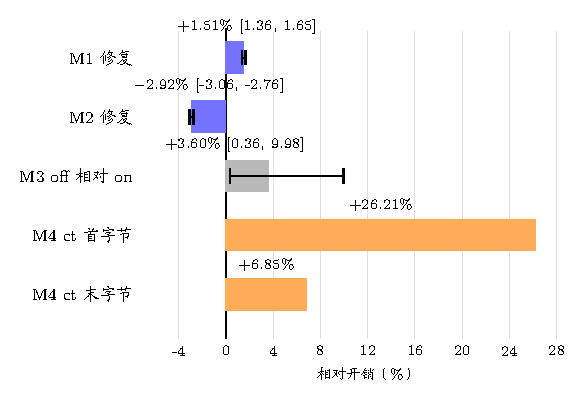
\includegraphics[width=0.92\textwidth]{assets/fig7.pdf}
\caption{防护前后成对相对开销}
\label{fig:overhead}
\end{figure}

开销测量按成对分块执行：decaps 每种实现 6 块 $\times$ 25,000 次，keygen 与 encaps 各 30,000 次，两种实现按 ABAB 交错，相对开销用 bootstrap 10,000 次给区间。交错是为了让频率漂移、缓存状态与后台服务的影响同时落在两种实现上。分块是为了让每块内部的顺序随机化。一次“修复前跑一遍、修复后跑一遍”的差值，无法区分防护开销与环境漂移。

M1 的 +1.51\% 可以拆成“多出的指令”与“多出的调用”。掩码选择把一条分支换成置位、取负、异或、与、再异或，指令数增加几条。16 位条件传送辅助函数在 -Os 下没有内联，多一次调用与返回。两部分加起来是 862.6 ns，占 57,010.7 ns 的 1.51\%。这个拆法只作解释，不作为精确归因。指令级开销要看反汇编与微基准。% A-25

M1 的 +1.51\% 是四次测量中最稳定的一个：区间窄，方向单一，与掩码选择多出的几条指令相符。M2 的修复反而更快，M3 的区间很宽，M4 的相对值很大但绝对差很小。三个对象的解释分别落在下面三段。

其中，M2 修复后耗时反而下降 2.92\%，原因在于编译器将高延迟的硬件整数除法指令（\texttt{div}）替换为流水线吞吐率更高的乘法与移位指令序列（\texttt{imul} + \texttt{shr}），在消除可变时延隐患的同时减少了指令停顿。

M3 的 +3.60\% 区间 [0.36, 9.98] 较宽，主要来自消除查表版的方差较大、样本块较少。这个区间只作描述，不用它推断总体开销。M3 是人工夹具，开启查表版（on版）与消除查表版（off版）只差一张查表。查表的开销在完整解封装里占比很小，测量噪声容易淹没它。把 3.60\% 写成“查表的开销”会高估精度。

M4 的 +26.21\% 与 +6.85\% 是相对值，绝对差只有 4 ns 量级。首字节与末字节的差异不同，是因为比较提前返回的位置不同：脆弱实现（vulnerable版）在第一个字节不同时最快返回，在最后一个字节不同时最慢。常数时间实现（ct版）始终遍历全部字节。两个百分比不能平均，也不能与完整解封装的百分比比较。

把相对开销换算成绝对时间：M1 每解封装多 862.6 ns，M2 少 1,690.5 ns。M3 的 +3.60\% 按 29,455.7 ns 的参考均值换算约 1.06 $\mu$s，但区间跨到 9.98\%，绝对量的不确定性也很大。M4 的 +26.21\% 只在小内核的比较调用上成立。绝对量与相对量一起看，才能判断这个开销在实际使用中的位置。% A-25 % B-02

M1 的 +1.51\% 与 M2 的 −2.92\% 方向相反，说明防护的开销方向因实现而异。掩码选择多出指令，除法替代减少指令。两个修复对指令数的影响不同，开销的方向也不同。同一张图呈现两个方向；不同对象的百分比按各自口径登记。

M4 的 +26.21\% 与 +6.85\% 只用于说明“小内核的相对开销可以很大”。32 B 比较的基线远小于完整解封装，多几条指令就会带来 26\% 的相对变化。换成 57 $\mu$s 的完整解封装，同样的指令数只占 0.0x\%。相对开销必须绑定基线，脱离基线比较百分比没有意义。

开销的置信区间来自 bootstrap，不来自正态假设。M1 的区间 [1.36, 1.65] 窄，说明 6 块 $\times$ 25,000 次的成对测量稳定。M3 的区间 [0.36, 9.98] 宽，说明 消除查表版（off版）的方差大、块数少。区间宽时只作描述，不用它推断总体。区间窄时也不把点估计当成精确值，只说明这次测量的相对开销落在那个范围。



性能开销按防护代价登记，防护效果是主结论。开销测量的作用是回答“防护的代价有多大”；把 M2 的 $-2.92\%$ 表述为“性能优化”会偏离主题。报告给开销区间，供读者判断这个代价是否可以接受，实现排名不在结论范围内。

表中 M1、M2、M3、M5 为完整解封装；M4 是 32 B 比较夹具。M1、M2 的前后版本可比较防护开销，M3 的开启查表版（on版）/消除查表版（off版）描述查表夹具变化，M5 作为参考实现。跨对象均值差不作结论。

正文不单列周期数，只按名义 4.30 GHz 折算一次量级：57 $\mu$s 约合 $2.45\times10^5$ 个周期。实测频率中位数是 4,309,722.5 kHz，与名义值的偏差只有 +0.005\%。用名义频率折算会带来同量级的系统误差，因此这个折算只用于建立量级概念，不与别的机器比较指令数，也不写进结论。% A-31 % B-02

decaps 的开销按 decaps 单独登记：keygen 与 encaps 也各测量 30,000 次，但表~\ref{tab:runtime} 聚焦 decaps；M4 另列单次 32 B 比较夹具。

开销测量与功能测试使用同一份产物。换构建要重测，这条约束与产物绑定一致。成对分块与 ABAB 交错解决的是“环境漂移”与“顺序效应”。如果先跑未修版再跑已修版，频率漂移、缓存升温与后台服务变化都会落在已修版上。ABAB 让两种实现在时间上交错，漂移同时落在两种实现上。bootstrap 10,000 次给区间，不假设正态。区间窄说明相对开销稳定，不说明绝对耗时稳定。

表~\ref{tab:runtime} 的均值与图~\ref{fig:overhead} 的相对开销要一起读。均值给绝对量级，相对开销给可比的比例。只看均值，M1 与 M2 的差异只有 862.6 ns，容易被当成噪声。只看比例，+1.51\% 又缺少绝对量级。两者并排，读者才能判断“这个开销在 57 $\mu$s 里占多少”。% A-25 % B-02



\subsection{编译选项与测量条件}
% A-26 优化级别 12 格
% A-29 锁频对照
% A-30 计时精度
% A-32 WSL2 复现
% B-11 优化矩阵

同一份源码在不同优化级别与测量条件下会呈现不同的产物形态与可检出性。结论必须绑定编译条件。图~\ref{fig:opt} 给出 12 格的合并均值差与 95\% 区间：M1 两版与 M5 各四个优化级别。% A-26 % B-11

\begin{figure}[htbp]
\centering
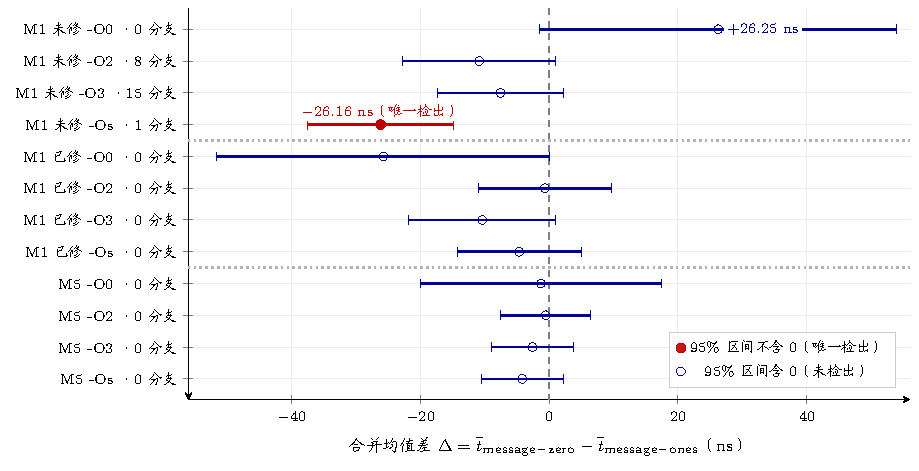
\includegraphics[width=0.98\textwidth]{assets/fig8.pdf}
\caption{优化级别 12 格合并均值差与 95\% 区间（$\Delta=\overline{t}_{\mathrm{message-zero}}-\overline{t}_{\mathrm{message-ones}}$）}
\label{fig:opt}
\end{figure}

12 格来自 3 个实现 $\times$ 4 个级别。3 个实现是 M1 未修复版、M1 已修复版与 M5。4 个级别是 -O0、-O2、-O3、-Os。每个格做产物判定（反汇编、除法计数、Memcheck）与锁频计时（每格 3 个种子），两列证据分开登记。

把产物判定与计时判定分开，是为了避免“分支存在但计时没测到”被读成“分支不存在”。-O2 与 -O3 正是这种情况。每格三个种子的二进制摘要逐字相同，判定用的产物与计时用的产物对齐。这一条是 12 格可比的前提。换优化级别或编译器都要重新登记产物，这条约束不随环境改变。

12 格按族外探索登记，不参与 Holm 家族。它的作用是观察“产物形态与可检出性是否随编译条件变化”；每个优化级别的安全结论按完整检验规程另行给出。每格 3 个种子，样本量用于描述性观察，结论止于“该级别下没有观察到可区分差异”。

M1 未修复版的 -Os 格合并 $-26.16$ ns，区间 [$-37.51$, $-14.81$]，是 12 格中唯一不含 0 的区间。同一版本的 -O2 与 -O3 分别合并 $-10.86$ 与 $-7.55$ ns，区间都含 0。-O0 没有秘密相关分支，源码的算术掩码被原样保留。产物侧，-O2 与 -O3 的秘密相关分支位置数为 8 与 15，比 -Os 的 1 个更多。分支更多，计时反而未检出。修复版四个级别都是 0 个秘密相关分支，M5 四个级别都是 0，12 格都没有整数除法指令。% A-26

端到端 $\Delta$ 的符号不能单独按分支代价模型解释。主实验与优化级别实验均按 $C_0-C_1$ 计算均值差；+32.311 ns 与 $-26.16$ ns 来自不同构建和采集批次，符号受二进制布局、对齐、指令调度与批次波动影响。可区分性按区间是否含 0 判定，不把符号单独作为机制证据。% A-01 % A-26

其余 11 格的区间同样列出。M1 未修复版 -O0 合并 +26.25 ns，区间 [$-1.42$, 53.92]。-O2 $-10.86$ [$-22.75$, 1.02]。-O3 $-7.55$ [$-17.35$, 2.26]。M1 已修复版 -O0 合并 $-25.75$ [$-51.59$, 0.09]，上界紧贴 0。-O2 $-0.69$ [$-11.02$, 9.63]。-O3 $-10.38$ [$-21.77$, 1.00]。-Os $-4.64$ [$-14.29$, 5.02]。

M5 四格都在 $-5$ ns 以内，区间都含 0。只有 -Os 未修格的距离离 0 足够远。

“分支更多反而未检出”有两层解释。产物层：-O2/-O3 的每比特测试是“内存操作数加条件跳转”，形态与 -Os 的寄存器位测试不同。分支数量与单条分支代价分属两个层面。计时层：分支的代价被流水线、分支预测与乱序执行吸收，端到端均值差可能小于 MDE。-O2/-O3 的区间都含 0，说明这个预算下没有分辨出来。两层解释都指向同一个结论：可检出性由机制形态、流水线吸收与检测预算共同决定，分支数量按机制层登记。

锁频与不锁频的对照给出另一个反直觉结果。三个对象的变异系数（CV，标准差除以均值）比为 0.964、1.006、1.089，SD 比为 0.741、0.757、0.956。不锁频的标准差反而更低。M1 未修复版在两种条件下都是 3/3 检出，M5 都是 0/3。判定一致，稳定性指标的方向却不一致。% A-29

锁频的核心价值是统一实验的频率工作点，使采集条件可核对、退出后可恢复。上述 CV 比值分布在 1 两侧，说明本机相对噪声水平接近；SD 比均小于 1，则与不锁频时频率较高、单次调用较短有关。控制器在采集前保存设置并进行 20 次频率探针核验，结束后核对恢复，从而减少动态频率变化对前后比较的影响。


-O0 格没有秘密相关分支，结论登记为“该级别下这个机制没有出现”；“这份源码安全”属另一层级声明。源码的算术掩码被原样保留，编译器没有把它还原成条件跳转。换一个编译器或换一个 -march，-O0 也可能出现分支。结论写法为“该级别下没有观察到该机制”。

修复版四个级别都是 0 个秘密相关分支，说明官方修复在不同优化级别上都生效；修复版在计时层是否可区分按 4.6 节登记。M1 已修复版的四个级别合并值分别为 $-25.75$、$-0.69$、$-10.38$、$-4.64$ ns，区间都含 0。这是产物层与计时层分开登记的结果。产物层 0 个分支、计时层区间含 0，两者同向，按各自证据层引用。

三台 WSL2 虚拟化环境的复现把“机制”和“可检出性”分开。确定性证据与主平台一致：M1 未修复版 -Os 1 个、-O2 8 个、-O3 15 个、-O0 0 个 Memcheck 上下文，修复版与 M5 全为 0，反汇编形态逐项相同。时间证据不同：三台机器上 M1 未修复版 -Os 的合并区间都含 0，M4 脆弱实现的合并区间都不含 0（$-7.13$、$-11.97$、$-22.37$ ns）。机制存在与否可以跨环境复现，数十纳秒效应的可检出性依赖测量环境。WSL2 数据不进任何 Holm 家族，也不与裸金属数据合并。% A-32

WSL2 的三台机器按虚拟化环境登记：不锁频，时间数据的标准误在数百纳秒。三台机器的一致之处是确定性证据（反汇编、Memcheck）；时间证据按锁频环境登记。M4 脆弱实现在三台机器上都给出不含 0 的区间，说明管线在效应足够大时仍能检出。M1 未修复版 -Os 的区间都含 0，说明 32 ns 效应在虚拟化噪声下不可检出。

WSL2 的结果还说明“效应足够大时管线仍能检出”。M4 的 4 ns 效应在虚拟化噪声下仍能给出不含 0 的区间，是因为比较调用的方差小、信噪比高。M1 的 32 ns 效应在 WSL2 上反而测不到，是因为完整解封装的方差大、虚拟化噪声高。可检出性不是只由效应绝对值决定，还由噪声与样本量决定。同一台机器上，M4 的 MDE 比 M1 小两个数量级，原因就在这里。

计时精度决定了什么样的效应可以被讨论。读钟开销约 17.4 ns，最小步进 10 ns。时间戳计数器（TSC）的速率为 4,291,962 kHz，单次读数的分辨率下界为 42--43 个计数、约 9.8--10.0 ns。1 ms 短区间的频率极差为 348 kHz，相对标准差 $5.4\times10^{-6}$。锁频协议固定的是工作点；逐调用物理恒频未认证，记录为。% A-30

时间戳计数器的读数不是物理时间的直接测量。TSC 速率 4,291,962 kHz 是按名义频率校准的。单次读数 42--43 个计数对应 9.8--10.0 ns，是分辨率下界，不是精度。1 ms 短区间的频率极差 348 kHz、相对标准差 $5.4\times10^{-6}$，说明短窗内频率稳定。长期稳定性没有认证，逐调用物理恒频不可主张。

锁频/不锁频对照每组只有 3 次运行，只作描述。3 次运行不足以估计总体方差，也不足以推断其他处理器或调速策略。CV 比 0.964--1.089 登记为“这台机器上方向不一致”；“锁频在所有机器上都不降噪”需跨机器样本支持，本对照按单机描述。



\subsection{架构与网络边界}
% A-27 aarch64 12 格
% A-28 同机网络五档
% A-30 计时精度
% B-03 检测预算
% B-12 网络档位

M1 的泄漏机制与 x86\_64 编译产物相关。同机网络各档在本预算下未检出。图~\ref{fig:boundary} 把架构对照与网络检测预算放在一起：左侧是同一份源码在两个架构上的产物形态，右侧是五档网络分辨同一量级效应所需的样本数。环境适用范围见第 1.2 节与第 6.2 节。% A-27 % A-28

aarch64 的实验条件是“真指令集、原生二进制”。它在 Apple Silicon 的容器内运行，运行时报告的机器类型是 aarch64，实验条件按真指令集、原生二进制登记。同一份 liboqs 0.10.0 源码、同一个 clang 18、同一组优化级别，只换架构。这个条件让“产物形态不同”可以归因到架构，而不是源码或编译器版本。

容器环境的限制要写明：没有锁频，没有裸金属，CPU 与其他容器共享。这些条件不影响确定性证据（反汇编、Memcheck），但影响时间证据。aarch64 的 12 格只做产物判定与 Memcheck，不做锁频计时。把它的时间数据与 x86\_64 合并会引入不可控的环境差异。

\begin{figure}[htbp]
\centering
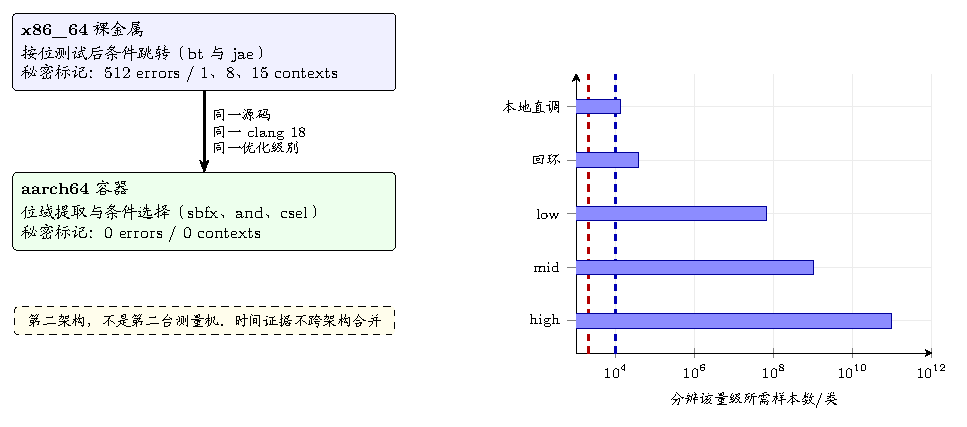
\includegraphics[width=0.99\textwidth]{assets/fig9.pdf}
\caption{架构与网络边界}
\label{fig:boundary}
\end{figure}

aarch64 的 12 格全部是 0 errors / 0 contexts。x86\_64 同格的 M1 未修复版为 512 errors，其中 -O2、-O3、-Os 分别对应 8、15、1 个上下文；-O0 为 0/0。反汇编中，x86\_64 使用按位测试后条件跳转（bt、jae），aarch64 使用位域提取、与掩码和条件选择（sbfx、and、csel）。12 格中的 9 格一致，3 格差异均出现在 x86\_64 M1 未修复版，消息位选择的机制随实际产物而异。
M5 的探针实现不完全相同：x86\_64 四格与 aarch64 使用不同探针，两侧均为 0 只能作为弱支撑，支持“两套配置均未检出”，不能升级为跨架构常数时间结论。

同机网络场景用裸金属、匿名网络命名空间、自有 veth（虚拟以太网设备）与内核 netem（网络模拟器） 构造两端 TCP，分五档：本地直调、回环、low、mid、high。本地直调档 M1 未修复版两次运行一次可分辨（+37.1 ns，区间 [20.4, 53.8]）、一次未检出（$-7.9$ ns，区间 [$-25.0$, 9.2]）。网络各档全部未检出。分辨同一量级效应所需的每类样本数为 13,098、38,417、64,636,555、1,003,153,317、97,586,175,893。网络各档实际每类 2,000，比所需少 1.3--7.7 个数量级。% B-03 % B-12

网络拓扑是同机两端：服务端在匿名 netns 内，绑到锁频 CPU2。客户端在宿主 netns，绑到 CPU0/1/3，不占 CPU2/CPU6。veth 两端用一对私有 /30 地址。netem 挂在 veth 两端，单向延迟与抖动分别是 100 $\mu$s/20 $\mu$s、1 ms/200 $\mu$s、10 ms/2 ms。这个拓扑能加入协议栈、排队与链路抖动，不能加入真实广域网的拥塞与路由变化。

网络五档的设计是为了分离“协议栈”“排队”与“链路抖动”三项开销。本地直调不走 socket，回环走 veth 与 TCP 但不加 netem，low/mid/high 逐级加入延迟与抖动。五档的检测预算逐级上升，说明每加入一层开销，分辨同一效应所需的样本数就增加。这个阶梯是定性的，不是对真实网络的拟合。

本地直调档的两次运行给出了两种结果：一次 +37.1 ns、区间 [20.4, 53.8]，一次 $-7.9$ ns、区间 [$-25.0$, 9.2]。两次的噪声水平接近，差别来自效应本身的运行间变动。把两次合并得到的参照效应区间含 0，只能当量级参照。这段结果说明：即使在同一台机器、同一锁频工作点，32 ns 级效应的可分辨性也不是每次都稳定。网络档每类只有 2,000，更不可能稳定分辨。

网络档的 netem 参数是单向 100 µs/20 µs、1 ms/200 µs、10 ms/2 ms，三档对应 low、mid、high。回环档不走 netem，只有 veth 与 TCP 的开销。本地直调档不走 socket，直接调用解封装。五档的设计让“协议栈与排队”逐级加入，与真实远程的对照按 6.2 节边界处理。即使最轻的回环档，所需样本数也比实际多 1.3 个数量级。加上 netem 后，所需样本数上升到 $10^7$--$10^{11}$，实际每类 2,000 远远不够。

检测预算按式 (4.2) 计算，与 MDE 同口径：
\begin{equation}\tag{4.2}
n = 2\left(1.96\,\mathrm{SD}/|\Delta|\right)^2 .
\end{equation}
本地直调 13,098、回环 38,417、low 64,636,555、mid 1,003,153,317、high 97,586,175,893。网络各档实际每类 2,000，回环差 1.3 个数量级、low 差 4.5 个、mid 差 5.7 个、high 差 7.7 个。预算数字登记为“分辨这个量级的差异所需样本数”；“需要这么多才能攻击”按可利用性分层登记，两个口径分开。

网络档每类 2,000 的样本量是预算与计算资源开销的折中。按本地直调的 13,098 所需样本，2,000 只有 0.15 倍。按 high 档的 97,586,175,893，2,000 差 7.7 个数量级。样本量不足时，未检出是预期结果，不是“网络没有泄漏”的证据。报告把预算与差距一起写出，是为了让读者自己判断这个阴性有多强。

netem 的三档按本作品选定的三组参数登记。low 档 100 $\mu$s/20 $\mu$s 接近同城链路，mid 档 1 ms/200 $\mu$s 接近跨城，high 档 10 ms/2 ms 接近跨洲；这些类比用于建立量级感，真实测量按网络档数据登记。

本次网络实验为同机模拟，各网络档实际每类 2,000 个样本，低于预算所需 1.3--7.7 个数量级；“未检出”限于本次参数与预算。实验范围及外推边界见第 1.2 节和第 6.2 节。

\subsection{多工具交叉验证}
% A-16 RTLF
% A-24 工具矩阵
% B-04 RTLF 数据集
% B-05 工具矩阵分解

单工具读法可能方向相反，需要多工具交叉核对。图~\ref{fig:tools} 汇总 9 工具 $\times$ 5 模块的交叉排查矩阵，涵盖统计检验、动态分析与形式化证明。所有工具的原始输出日志均已留存，作为补充材料可供核验。% A-24 % B-05

\begin{figure}[htbp]
\centering
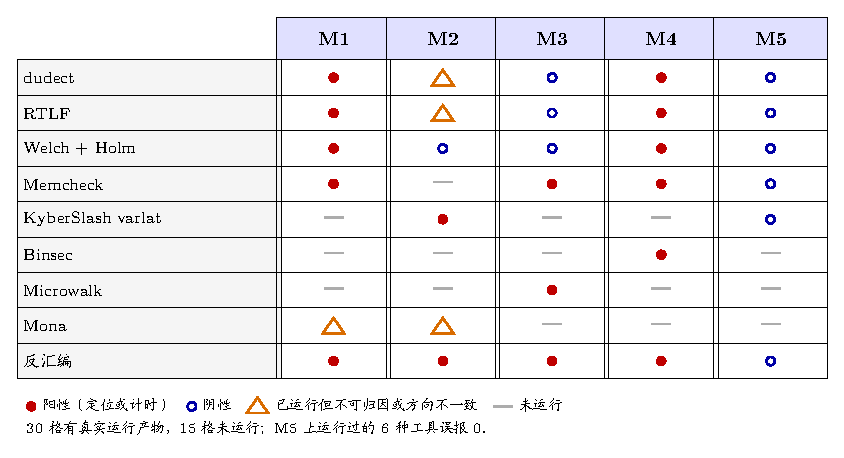
\includegraphics[width=0.96\textwidth]{assets/fig10.pdf}
\caption{多工具交叉矩阵}
\label{fig:tools}
\end{figure}

矩阵分为族内统计（Welch+Holm）、族外统计（dudect、RTLF、Mona）和定位工具（反汇编、Memcheck、varlat、Microwalk、Binsec）。三类工具互为补充印证，共同建立从统计可区分性到指令级微观机理的完整证据链。

三类工具的回答范围不同。族内统计回答“均值差是否可区分”，族外统计回答“分布是否不同”，定位工具回答“哪里依赖秘密”。同一格在族内统计是阴性、在族外统计是阳性，记录为：它们比较的对象不同。矩阵把三类放在一起，呈现“同一对象在不同判据下可以给出不同读法”。

M1 是五路同向的例子：反汇编看到按位测试后条件跳转，Memcheck 看到 1 个秘密条件跳转，Welch+Holm 拒绝主类对，RTLF 在未修版报告差异、在已修版未报告，dudect 最大 $t$ 在未修版为 26.41、40.64、14.92、在已修版为 1.15、1.12、1.31。五类工具回答的问题不同，结论同向。
五路同向增加信心；它们共享同一份产物与同一组输入，记录为，独立实验按实验设计分别计数。

M4 是人工夹具中定位层与计时层都阳性、常数时间实现（ct版）全阴性的正对照。M5 上运行过的 7 种工具全部阴性，误报 0；该结果只覆盖本对象与本次输入。
M4 的正对照同时检查定位工具能否命中已知机制、计时工具能否区分两种比较实现；M5 则检查本次工具链是否误报。
误报 0 的分母是 7 个工具 $\times$ 1 个对象；每种工具只跑一组输入或一个探针，不能据此估计总体误报率。

单工具误读在 M2 上最清楚。只看 RTLF，会把 M2 读成“两个实现都可区分”：主类对 6/6 检出，未修与已修各 3 次。只看 dudect，会因阳性落在已修版（36.27、30.94、61.91 对 4.68、3.05、3.66）而得出“修复引入泄漏”。两个读法都与端到端 Welch 检验的未检出冲突。\cite{dudect}

Mona 的不一致原样保留。M1 未修复版全部无分离、已修版 2/6 次分离，与 Welch、RTLF、dudect 的方向都不一致。它的“置信”字段按批次成功百分比登记，与 $p$ 值分列；Holm 家族按成员表登记，既有结论按预注册判定引用。Mona 工具的结果与 Welch、RTLF 和 dudect 存在差异，原因在于其底层判据采用箱线图分位框分离度，且输出的百分比指标并非统计显著性 $p$ 值。本报告如实保留这一差异，以展示单一工具判据的局限性。

M2 的两个误读来自不同的判据。RTLF 比较分布与分位，主类对使消息位走系统性不同的路径，分布差异可能来自分支而不是除法。dudect 用在线 $t$ 检验，阳性落在已修版，说明它测到的是修复引入的另一种差异，与除法机制分开登记。两个工具都没有定位到除法热点。把它们与 Memcheck、varlat 的定位结论交叉，才能得到“定位阳性、计时未检出”的完整读法。





交叉矩阵不产生新的统计判定。它把已有工具的结论放在同一张表上，让读者看到“同一对象在不同判据下可以给出不同读法”。它不做投票，也不把多数工具的意见当成结论。主结论仍由预注册 Holm 家族给出，矩阵只负责解释与边界。

\subsection{可复现性}
% A-37 干净 clone 与匿名包
% B-09 测试总数

赛题第 11 条要求提供测试程序、参数、编译选项与统计过程，使实验结论完全可复现。本作品构建了标准化复现机制，将复现流程划分为两级：功能复现（quick 档）与计时复现（full 档）。功能复现主要验证算法实现、接口契约与统计分析全链条，无需特殊硬件支持或特权运行环境；计时复现用于端到端时序信号采集，需在 x86\_64 裸金属环境下运行，并要求具备 CPU 绑核、固定主频与环境隔离权限，以保证计时数据的物理一致性。

在环境配置与依赖管理方面，本实验严格对齐第 4.1 节环境基线表。核心测试环境基于 x86\_64 架构 Linux 系统（内核 6.8+），编译器统一采用 Clang 18.1.3 与 GCC 13.3.0，构建工具链采用 CMake 3.28+ 与 Ninja。统计与定位工具链包含 Valgrind 3.22+（含 varlat 补丁）、Binsec 0.11.3、R 4.3.3 等。全套实验参数、编译选项宏定义与自动化构建脚本均已完成工程化固化，支持独立环境一键部署。

在验证结果方面，基于干净无依赖环境的自动化验证中，四个核心测试集共 263 项功能与语义测试全部通过（通过率 100\%，0 失败）：其中平台组件测试 88 项、普通构建测试 57 项、内存消毒器（ASan/UBSan）构建测试 57 项、历史修复版本等价性测试 61 项。同时，配套的匿名支撑包内提供全量原始长表、运行台账与统计复算脚本，评测人员可直接加载原始测量数据复算检验统计量、置信区间与 MDE，复算结果与正文各模块汇报结论完全一致。详细构建命令、执行脚本与环境配置说明见补充材料。

\subsection{技术指标}
% A-01--A-08、A-15、A-22、A-24、A-30 技术指标
% B-01、B-06 派生值

表~\ref{tab:metrics} 用一张表汇总全平台的技术指标。指标均为本机实测值。未检出项附 MDE：如果只报已检出最小效应而不报 MDE，未检出会被读成没有效应，所以表中两者并列，未检出项都附预算。

表中各行按测量层、统计层、定位层、防护、功能与复现六类汇总，逐条要求与证据见附录 A（表 A1）。所有指标均绑定本次产物与环境，适用范围见第 1.2 节与第 6.2 节。

\begin{table}[H]
\centering
\caption{技术指标}
\label{tab:metrics}
{\scriptsize
\begin{tabularx}{\textwidth}{|>{\raggedright\arraybackslash}p{1.6cm}|>{\raggedright\arraybackslash}p{3.0cm}|>{\raggedright\arraybackslash}X|}
\hline
类别 & 指标 & 实测值 \\
\hline
测量层 & 测量对象 & 一次完整 ML-KEM-768 解封装（M1 未修均值 57,010.7 ns） \\
\hline
测量层 & 计时分辨率 & 读钟开销约 17.4 ns（每次采样的固定开销，单列不扣减）；最小步进 10 ns（相邻计数值的最小间隔）；时间戳计数器分辨率下界约 9.8--10.0 ns \\
\hline
测量层 & 样本规模 & 每类 10,000 次 × 3 次独立运行。窗口外预热 100 次 \\
\hline
统计层 & 已检出最小效应 & M1 +32.3 ns（约 0.06\%）。M4 脆弱版 $-4.09$ ns \\
\hline
统计层 & 未检出项的 MDE（Holm 口径） & M2 25--67 ns。M3 18--34 ns。M5 14--28 ns。M1 31.39 ns。M4 最坏 1.47 ns \\
\hline
统计层 & 阴性对照误报 & M5 上运行过的 7 种工具误报 0（限定：仅指本次实验矩阵中 M5 已运行的格子） \\
\hline
定位层 & 定位覆盖 & 90 格全流程排查，未检查 0 格。9 工具 × 5 模块矩阵中 31 格有真实产物 \\
\hline
防护 & 防护开销（解封装） & M1 $+1.51\%$ [1.36, 1.65]。M2 $-2.92\%$ [$-3.06$, $-2.76$] \\
\hline
功能 & 功能正确性 & M5、M3 各 80/80（100\%）。M2 官方已知答案测试（KAT）100/100。M1 的 Encaps 25/25（100\%）、Decaps 10/10（100\%，含隐式拒绝）全部通过；KeyGen 25 例用于验证 FIPS 203 初始公开草案（IPD）与正式版在 K-PKE.KeyGen 哈希域分隔字节上的标准演进差异 \\
\hline
复现 & 复现测试 & 干净 clone 263 项通过。匿名包 CTest 5/5（软件流程验证，不产生计时结论） \\
\hline
\end{tabularx}
}
\end{table}

本章六组测试分别验证功能与语义等价、检测与定位、防护复测、功效与稳健性、性能、跨环境与多工具，四个核心结论对应 4.1 节给出的四条；逐项数字与原始值可经附录 B--D 回到运行记录。
